% Created 2021-01-24 Sun 22:49
% Intended LaTeX compiler: pdflatex
\documentclass[11pt]{article}
\usepackage[utf8]{inputenc}
\usepackage[T1]{fontenc}
\usepackage{graphicx}
\usepackage{grffile}
\usepackage{longtable}
\usepackage{wrapfig}
\usepackage{rotating}
\usepackage[normalem]{ulem}
\usepackage{amsmath}
\usepackage{textcomp}
\usepackage{amssymb}
\usepackage{capt-of}
\usepackage{hyperref}
\usepackage{minted}
\hypersetup{colorlinks=true, linkcolor=black, filecolor=red, urlcolor=blue}
\usepackage[turkish]{babel}
\author{Eren Hatırnaz}
\date{1 Mart 2020}
\title{Yazılım Gündemi - 2020/08\\\medskip
\large 17 Şubat - 1 Mart 2020}
\hypersetup{
 pdfauthor={Eren Hatırnaz},
 pdftitle={Yazılım Gündemi - 2020/08},
 pdfkeywords={},
 pdfsubject={},
 pdfcreator={Emacs 27.1 (Org mode 9.3)},
 pdflang={Turkish}}
\begin{document}

\maketitle
\tableofcontents \clearpage\shorthandoff{=}

\begin{center}
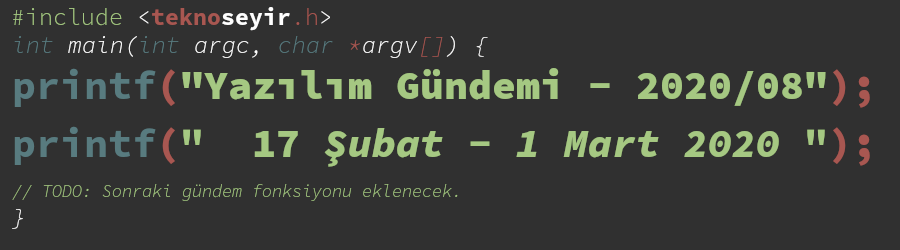
\includegraphics[width=.9\linewidth]{gorseller/yazilim-gundemi-banner.png}
\end{center}

\begin{center}
\href{../07/yazilim-gundemi-2020-07.pdf}{< Önceki Gündem} | \textbf{17 Şubat - 1 Mart 2020} | \href{../09/yazilim-gundemi-2020-09.pdf}{Sonraki Gündem >}

\href{https://teknoseyir.com/blog/yazilim-gundemi-2020-08}{TeknoSeyir'de Oku}
\end{center}

\section{Son 13 yılın tüm Apache Tomcat sürümlerini etkileyen \href{https://www.zdnet.com/article/ghostcat-bug-impacts-all-apache-tomcat-versions-released-in-the-last-13-years/}{güvenlik açığı ortaya çıktı}: \href{https://www.chaitin.cn/en/ghostcat}{Ghostcat}}
\label{sec:orgd7bb6ef}
\begin{figure}[htbp]
\centering

\includegraphics[height=2cm]{gorseller/ghostcat.png}
\caption{Ghostcat Maskotu. Son yıllarda artık güvenlik açıklarının da maskotunun olması moda oldu.}
\end{figure}

Çinli siber güvenlik firması Chaitin Tech tarafından ortaya çıkan bu güvenlik
açığı sayesinde kötü amaçlı kişiler sunucunuzdaki dosyaları okuyabilir, hatta
bazı durumlarda ise yazabiliyor. 2007 yılından bu yana çıkmış bütün Apache
Tomcat versiyonlarını kapsayan bu açık Java ile geliştirilmiş web
uygulamalarını tehdit ediyor. Bulan araştırmacılar ise açığa "Ghostcat" ismini
vermişler. Açığın uluslararası kodu ise \href{http://cve.mitre.org/cgi-bin/cvename.cgi?name=CVE-2020-1938}{CVE-2020-1938}.

Aslında açığın asıl kaynağı Apache Tomcat'in içinde kullanılan bir AJP isimli
parçadan kaynaklanıyor. Açılımı Apache JServ Protocol olan bu parça, sunucunun
diğer Tomcat ya da Apache HTTPD sunucuları ile veri alışverişi yapabilmesine
yarıyormuş. Bu parça tüm Tomcat sunucularında varsayılan olarak açık geliyor
ve 8009 numaralı port üzerinden yayın yapıyor. Bu açık sayesinde hackerlar
sunucunuzun ayar dosyaları okuyup, bir takım hassas verileri çalabilirler.
Eğer sunucunuzda kullanıcıların dosya yüklemesini sağlayan bir mekanizma varsa
bu açık sayesinde kötü amaçlı kişiler sisteminize bir takım zararlı yazılımlar
da enjekte edebiliyorlar.

Açığı bulan firma ve Apache Tomcat birlikte çalışmışlar ve açığı kapatan sürüm
güncellemelerini yayınlamışlar fakat bu güncellemeler sadece \href{https://tomcat.apache.org/security-7.html\#Fixed\_in\_Apache\_Tomcat\_7.0.100}{Tomcat 7.x},
\href{https://tomcat.apache.org/security-8.html\#Fixed\_in\_Apache\_Tomcat\_8.5.51}{Tomcat 8.x} ve \href{https://tomcat.apache.org/security-9.html\#Fixed\_in\_Apache\_Tomcat\_9.0.31}{Tomcat 9.x} sürümleri için yayınlandı. Diğer sürümler
hayatlarının sonuna gelmiş (End of Life) oldukları için o sürümler için
güncelleme gelmeyecek.

Hangi sunucuların etkilendiğini tespit etmek güç olsa da BinaryEdge firmasına
göre yaklaşık bir milyondan fazla Tomcat sunucusu şu an internette yayın
yapmakta. Aynı zamanda Java ile web uygulama geliştirmeye yarayan Spring Boot
kütüphanesinin de bu açıktan etkilenenler \href{https://snyk.io/blog/ghostcat-breach-affects-all-tomcat-versions/}{arasında olduğu söyleniyor}.

Eğer sizin de Apache Tomcat üzerinden yayın yapan web uygulamalarınız varsa
en kısa zamanda son sürüme güncellemenizi şiddetle tavsiye ederim.
\section{Safari yakında 13 aydan uzun geçerliliği olan \href{https://thenextweb.com/security/2020/02/24/safari-will-soon-reject-any-https-certificate-valid-for-more-than-13-months/}{sertifikaları kabul etmemeye başlayacak}}
\label{sec:org919bbe8}
Apple ekosisteminin varsayılan tarayıcısı olan Safari, geçtiğimiz haftalarda
düzenlenen 49'uncu \href{https://cabforum.org/}{CA/Browser Forum}'unda yeni bir kural duyurdu: "Eğer
sertifikanın geçerlilik tarihi 13 aydan fazla (398 gün) ise reddedeceğim".
Yani demek oluyor ki web sitenizin HTTPS sertifikasını her yıl yenilemezseniz
Safari tarayıcısı kullanıcılarına "bu site güvenli değil" uyarısı gösterecek.

\begin{figure}[htbp]
\centering
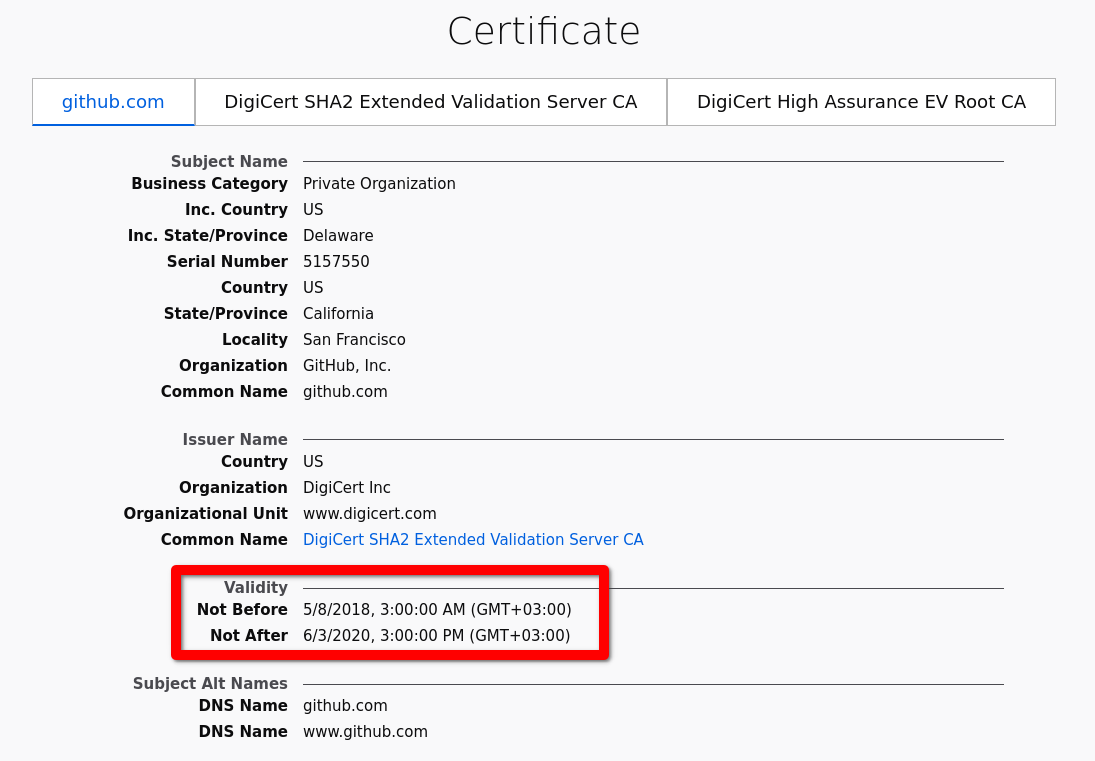
\includegraphics[height=6cm]{gorseller/safari-sertifika-github.png}
\caption{GitHub'ın güncel sertifika bilgileri}
\end{figure}
\begin{figure}[htbp]
\centering
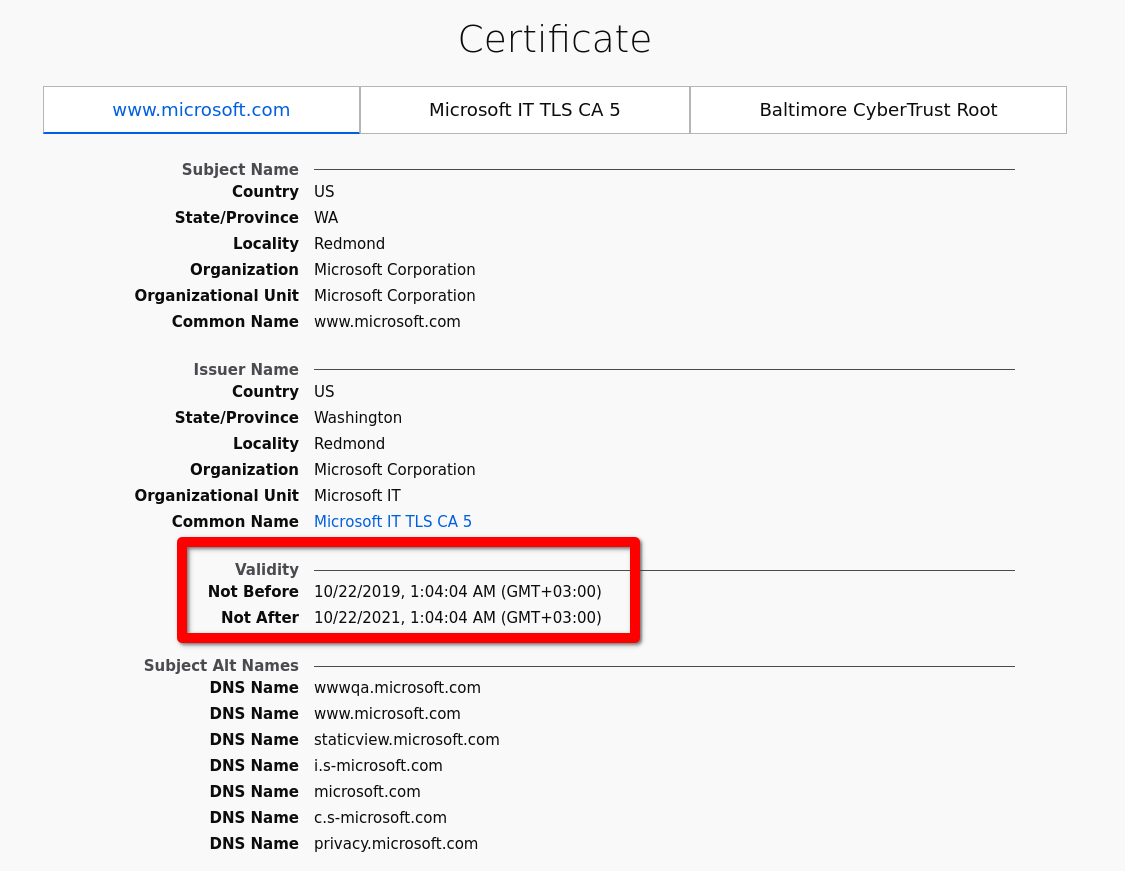
\includegraphics[height=6cm]{gorseller/safari-sertifika-microsoft.png}
\caption{Microsoft'un güncel sertifika bilgileri}
\end{figure}
\newpage

GitHub ve Microsoft gibi büyük şirketler de fazla uğraşmamak için HTTPS
sertifikalarını 2 yıllık alıyor. Eğer Safari bu kararından geri adım atmazsa
Microsoft ve GitHub da sertifikalarını yenilemek zorunda kalacak.

Safari'nin neden böyle bir karar aldığını anlamak güç. Let's Encrypt gibi
ücretsiz sertifika sağlayan otoritelerin otomatik yenileme araçları olsa da
diğer otoritelerin böyle bir çözümü var mı emin değilim. Sizler de Safari'nin
bu yeni kuralından etkilenmek istemiyorsanız aktif web sitelerinizin HTTPS
sertifikalarının geçerlilik sürelerini kontrol edin.
\section{GitHub Öğrenci Geliştirici Paketi 100+ ücretsiz \href{https://github.blog/2020-02-25-over-100-partners-to-help-you-succeed-with-the-github-student-developer-pack/}{servis ve araç sayısına ulaştı}}
\label{sec:org21aa480}
\begin{center}

\includegraphics[height=4cm]{gorseller/github-ogrenci-gelistirici-paketi.png}
\end{center}

GitHub'ın yaklaşık 6 yıl vermeye başladığı bu paket, bu hafta eklenen 14
teklifle birlikte 100'den fazla ücretsiz servis ve aracı öğrenci
geliştiricilerle buluşturmaya devam ediyor. Üniversiteniz size \textbf{.edu} ya da
\textbf{.edu.tr} ile biten bir mail adresi veriyorsa bu paketten siz de
yararlanabiliyorsunuz. \href{https://education.github.com/pack}{Bu adresten} paketi almak için başvuru yapabilirsiniz.
Genelde çok kısa bir süre içinde aktif oluyor paketiniz ve içerisinde
geliştirme yaparken kullanabileceğiniz birçok araç ve hizmet var. Ben de
üniversiteyken almıştım ve birçok avantajından faylanmıştım. Öğrenci
arkadaşların mutlaka göz atmasını ve paketi almalarını tavsiye ederim. Sektöre
hazırlık için çok faydalı olacak. Eğer üniversiteniz bu .edu ya da .edu.tr ile
biten e-posta adresi sağlamıyorsa gerekli mercilere başvurarak ısrarla
isteyiniz :)

Ayrıca bu hafta içerisinde GitHub'a çok satırlı kod önerme özelliği de \href{https://github.blog/changelog/2020-02-26-multi-line-code-suggestions-beta/}{beta
olarak yayınlandı}.
\section{.NET Core 3 sürümü 3 Mart'da \href{https://devblogs.microsoft.com/dotnet/net-core-3-0-end-of-life/}{emekliye ayrılıyor}}
\label{sec:org9b20a5b}
Microsoft'un açık kaynak olarak geliştirmeye devam ettiği .NET ekosisteminin
ana parçası olan .NET Core'un 3 numaralı sürümü 3 Mart'tan itibaren emekliye
ayrılıyor. Bu da demek oluyor ki bundan sonra .NET Core 3 sürümü için destek
sunulmayacak. Microsoft onun yerine geçtiğimiz aylarda LTS (Long-term
Support - Uzun dönemli destek) olarak duyurduğu 3.1 sürümüne geçmeyi tavsiye
ediyor.

Bu sürüm güncellemesini yapmak için \texttt{.csproj}, \texttt{.vbproj} ya da \texttt{.fsproj} ile
biten proje dosyasınızı açıp içerisindeki şu satırı:
\begin{minted}[breaklines=true,breakanywhere=true,frame=lines, linenos, label=XML, labelposition=topline]{xml}
<TargetFramework>netcoreapp3.0</TargetFramework>
\end{minted}
şununda değiştirebilirsiniz:
\begin{minted}[breaklines=true,breakanywhere=true,frame=lines, linenos, label=XML, labelposition=topline]{xml}
<TargetFramework>netcoreapp3.1</TargetFramework>
\end{minted}

Eğer hali hazırda .NET Core 3 ile çalışan bir uygulamanız varsa o kadar da
acele etmenize gerek yok fakat yavaş yavaş sürüm yükseltmeye hazırlanmanız
sizin için iyi olacaktır.
\section{VueJS Belgeseli yayınlandı}
\label{sec:org1380e19}
Popüler JavaScript kütüphanelerinden biri olan VueJS'in hikayesini
geliştiricisi Evan You ve katkı sağlayan diğer geliştiricilerinden ağzından
dinlemek için \href{https://www.youtube.com/watch?v=OrxmtDw4pVI}{şu YouTube videosunu izleyebilirsiniz}.
\section{Qt, Visual Studio Linux desteği için \href{https://devblogs.microsoft.com/cppblog/qt-to-support-visual-studio-linux-projects/}{çalışmaya başlamış}}
\label{sec:org1fae992}
C++ ile platformlar-arası uygulama geliştirmeye yarayan uygulama çatısı Qt
geçtiğimiz haftalarda yayınlandığı \href{https://www.qt.io/blog/cross-platform-development-with-qt-and-visual-studio}{blog yazısı}yla birlikte Visual Studio Linux
sürümü için de Qt desteği sunmak için çalıştıklarını duyurdu. İlk sürümününü
bu yılın yaz aylarında yayınlamayı planlıyorlarmış. Bu sayede zaten birçok
platform için destek sunan Qt, kapsamını daha da genişletmiş olacak.
\section{Yaklaşan Etkinlikler}
\label{sec:org9bebd89}
\begin{longtable}{|p{8cm}|l|l|}
\hline
Etkinlik İsmi & Yeri & Tarihi\\
\hline
\endfirsthead
\multicolumn{3}{l}{Önceki sayfadan devam ediyor} \\
\hline

Etkinlik İsmi & Yeri & Tarihi \\

\hline
\endhead
\hline\multicolumn{3}{r}{Devamı sonraki sayfada} \\
\endfoot
\endlastfoot
\hline
\href{https://www.eventbrite.com/e/yurt-dsnda-yazlmc-olmak-tickets-97277791493}{Yurt Dışında Yazılımcı Olmak!} & İstanbul & 2 Mart 18:30\\
\href{https://www.eventbrite.com/e/siber-guvenlik-ve-bt-denetiminde-kariyer-registration-96218045765}{Siber Güvenlik ve BT Denetiminde Kariyer} & İstanbul & 3 Mart 18:00\\
\href{https://www.meetup.com/DevTest-Community/events/269032606/}{Dealing with Errors on JVM with e} & İstanbul & 3 Mart 19:00\\
\href{https://kommunity.com/devops-turkiye/events/prometheus-ve-grafana-ile-metrik-olusturma-ve-goruntuleme}{Prometheus ve Grafana ile Metrik Oluşturma ve Görüntüleme} & İstanbul & 4 Mart 18:30\\
\href{https://www.meetup.com/AWS-User-Group-Turkey/events/268979622/}{AWS Meetup No.46 - AWS ve Güvenlik} & İstanbul & 4 Mart 19:00\\
\href{https://www.meetup.com/Microsoft-Giri\%25C5\%259Fimcilik-Bulu\%25C5\%259Fmalar\%25C4\%25B1/events/268504717/}{Microservice with Azure Kubernetes Service and Azure Devops} & İstanbul & 5 Mart 13:00\\
\href{https://www.eventbrite.com/e/nedir-bu-devops-dedikleri-tickets-95894584283}{Nedir Bu DevOps Dedikleri} & Ankara & 5 Mart 19:00\\
\href{https://www.meetup.com/Istanbul-Hackers/events/268983054/}{Private Kubernetes Cluster Automation with Terraform} & İstanbul & 5 Mart 19:00\\
\href{https://kommunity.com/fp-istanbul/events/functional-programming-istanbul-001}{Functional Programming Istanbul 001} & İstanbul & 5 Mart 19:30\\
\href{https://www.meetup.com/QWomen-\%25C4\%25B0stanbul/events/268233749/}{Kuantum Programlamaya Giriş Atölyesi} & İstanbul & 7 Mart 09:00\\
\href{https://www.meetup.com/gdgtekirdag/events/268421016/}{WTM Tekirdağ IWD 2020} & Tekirdağ & 7 Mart 10:00\\
\href{https://www.meetup.com/GDG-Cloud-Istanbul/events/268749560/}{Google Cloud Run Workshop} & İstanbul & 7 Mart 14:00\\
\href{https://www.meetup.com/rladies-ankara/events/269092053/}{Tanışma ve Kaynaşma Buluşması (R-Ladies Ankara)} & Ankara & 7 Mart 13:00\\
\href{https://www.meetup.com/GDG-Cloud-Izmir/events/268749612/}{GCP Projects, Service Account And Billing \& Intro to Computing in GCP} & İzmir & 8 Mart 13:00\\
\href{https://www.meetup.com/GDG-Manisa/events/268736708/}{Firebase Study Jam} & Manisa & 10 Mart 12:00\\
\href{https://www.meetup.com/gdg-cloud-ankara/events/269089185/}{Kubernetes'e Giriş StudyJam} & Ankara & 10 Mart 18:00\\
\href{https://kommunity.com/cloud-and-serverless-turkey/events/serverless-mindset-and-serverless-data-analytics-getir-ankara}{Serverless Mindset and Serverless Data Analytics} & Ankara & 12 Mart 18:30\\
\href{https://www.meetup.com/trendyol/events/268292201/}{Kotlin Reactive Programing-Coroutines} & İstanbul & 12 Mart 19:15\\
\href{https://www.meetup.com/Facebook-Developer-Circle-Istanbul/events/269082757/}{Containers for Java Devs - Mohammed Aboullaite} & İstanbul & 12 Mart 19:15\\
\href{https://www.meetup.com/Istanbul-Java-User-Group/events/268426411/}{Java Day Pre-Conference} & İstanbul & 13 Mart 13:00\\
\href{https://kommunity.com/devnot-yazilimci-bulusmalari/events/merkeziyetsiz-uygulamalardapps-gelistirme}{Merkeziyetsiz Uygulamalar(dApps) Geliştirme} & İstanbul & 13 Mart 19:00\\
\href{https://kommunity.com/btorgtr/events/test-bilisim-kahvesi-laboratuari}{Test: Bilişim Kahvesi Lab} & İstanbul & 13 Mart 19:30\\
\href{https://www.meetup.com/Istanbul-Java-User-Group/events/267956332/}{Java Day Istanbul 2020} & İstanbul & 14 Mart 08:00\\
\hline
\end{longtable}
\section{Diğer Haberler}
\label{sec:orgf5f2b67}
\begin{itemize}
\item Let's Encrypt, 1 milyar \href{https://letsencrypt.org/2020/02/27/one-billion-certs.html}{sertifika rakamına ulaştı}.
\item \href{https://www.jetbrains.com/company/annualreport/2019/}{JetBrains 20 yaşında}.
\item JetBrains, \href{https://surveys.jetbrains.com/s3/e4-kotlin-census-2019}{Kotlin Census 2019 Anketi}ni başlattı.
\item Microsoft, Koronavirüs nedeniyle Game Developer Conference 2020 \href{https://www.gematsu.com/2020/02/microsoft-cancels-gdc-2020-presence-due-to-coronavirus-concerns}{etkinliğini
iptal etti}. Facebook'da kendi geliştirici konferansını \href{https://www.theguardian.com/technology/2020/feb/27/facebook-f8-coronavirus-san-francisco-health}{aynı nedenle iptal
etti}. \href{https://esa-pages.io/p/sharing/68/posts/1006/b15a58c675f5a69d06e5.html}{RubyKaigi 2020} etkinliği de iptal edildi.
\item Facebook, deneysel Javascript araç kutusunu \href{https://twitter.com/sebmck/status/1232885861135421441}{açık kaynak olarak yayınladı}:
\href{https://github.com/facebookexperimental/rome}{Rome}.
\item Netflix, kriz yönetim sistemini \href{https://medium.com/NetflixTechBlog/introducing-dispatch-da4b8a2a8072\%0A}{açık kaynak hale getirdi}: \href{https://github.com/Netflix/dispatch}{Dispatch}.
\item Google, Cloud sistemi için monitörleme panellerinin \href{https://cloud.google.com/blog/products/management-tools/introducing-the-cloud-monitoring-dashboards-api}{API'sini duyurdu}:
\href{https://cloud.google.com/monitoring/dashboards/api-dashboard}{Stackdriver Cloud Monitoring dashboards API}.
\item Özgür Yazılım Vakfı, 2020 yılı içinde kendi kod barındırma platformunu \href{https://www.fsf.org/blogs/sysadmin/coming-soon-a-new-site-for-fully-free-collaboration}{ayağa
kaldıracağını duyurdu}.
\item JPEG komitesi yapay zeka bazlı resim sıkıştırma \href{https://jpeg.org/items/20200217\_press.html}{için çağrıda bulundu}.
\item Android Studio ve araçlarının yeni versiyonları yayınlandı:
\begin{itemize}
\item \href{https://androidstudio.googleblog.com/2020/02/android-studio-361-available.html}{Android Studio 3.6.1}
\item \href{https://androidstudio.googleblog.com/2020/02/android-studio-41-canary-1-available.html}{Android Studio 4.1 Canary 1}
\item \href{https://androidstudio.googleblog.com/2020/02/android-studio-40-beta-1-available.html}{Android Studio 4.0 Beta 1}
\item \href{https://androidstudio.googleblog.com/2020/02/emulator-3002-canary-haxm-756-and-amd.html}{Android Emulator 30.0.2, HAXM 7.5.6 ve Hypervisor 1.4}
\end{itemize}
\item TypeScript 3.8 Final \href{https://devblogs.microsoft.com/typescript/announcing-typescript-3-8/}{sürümü yayınlandı}.
\item Go programlama dilinin 1.14 \href{https://tip.golang.org/doc/go1.14}{sürümü yayınlandı}.
\item OCaml programlama dilinin 4.10 \href{https://discuss.ocaml.org/t/ocaml-4-10-released/5194}{sürümü yayınlandı}
\item Nim Topluluk Anketi 2019 \href{https://nim-lang.org/blog/2020/02/18/community-survey-results-2019.html}{sonuçları yayınlandı}.
\item Rust dili için \href{https://blog.rust-lang.org/inside-rust/2020/02/25/intro-rustc-self-profile.html}{profilleyici tanıtıldı}.
\item R programlama dili \href{https://twitter.com/\_R\_Foundation/status/1233671896144793600}{20 yaşında}.
\item CouchDB 3.0 \href{https://blog.couchdb.org/2020/02/26/3-0/}{sürümü yayınlandı}.
\item Swift takımı, \href{https://github.com/apple/swift-argument-parser}{ArgumentParser} kütüphanesini \href{https://swift.org/blog/argument-parser/}{duyurdu}.
\item Tech Debt Developer anketi \href{https://codeahoy.com/2020/02/17/technical-debt-survey/}{sonuçları yayınlandı}.
\item State of Clojure 2020 anketi \href{https://clojure.org/news/2020/02/20/state-of-clojure-2020}{sonuçları yayınlandı}.
\item C++ kütüphanesi EnTT, 3.3.0 \href{https://github.com/skypjack/entt/releases/tag/v3.3.0}{sürümünü yayınladı}.
\item IRedis aracının 1.2.0 \href{https://github.com/laixintao/iredis/releases/tag/v1.2.0}{sürümü çıktı}.
\item XMake v2.3.1 \href{https://tboox.org/2020/02/23/xmake-update-v2.3.1/}{sürümü yayınlandı}.
\item Scala.JS kütüphanesinin ilk stabil \href{https://www.scala-js.org/news/2020/02/25/announcing-scalajs-1.0.0/}{sürümü 1.0.0 çıktı}.
\item Tarayıcı üzerinde çalışan metin editörü \href{https://edtr.io/blog}{edtr.io tanıtıldı}.
\end{itemize}
\section{Lisans}
\label{sec:orgb41b595}
\begin{center}
\begin{center}

\includegraphics[height=1.5cm]{../../../img/CC_BY-NC-SA_4.0.png}
\end{center}

\href{yazilim-gundemi-2020-08.pdf}{Yazılım Gündemi - 2020/08} yazısı \href{https://erenhatirnaz.github.io}{Eren Hatırnaz} tarafından \href{http://creativecommons.org/licenses/by-nc-sa/4.0/}{Creative Commons
Atıf-GayriTicari-AynıLisanslaPaylaş 4.0 Uluslararası Lisansı} (CC BY-NC-SA 4.0)
ile lisanslanmıştır.
\end{center}
\end{document}
